% -*- root: ../GeometriaDiferencial.tex -*-
\chapter{Teorema de Gauss-Bonnet}
\label{chapGaussBonnet}

\section{Introducción y motivación}

El último tema del curso va a tratar de formalizar una idea que ha asomado la cabeza en temas anteriores: la conexión entre la topología y la geometría. Por ejemplo, con el Lema de Poincaré (\ref{thmPoincare}) veíamos que, de algún modo, las formas diferenciales ``veían'' el espacio en el que estaban definidas. La cohomología de De Rham (\ref{defCohomologiaDeRham}) también nos daba pistas de esa relación entre geometría y topología.

La cuestión es que hay una relación todavía más profunda entre ambas. Esta relación es la que se materializa con el teorema de Gauss-Bonnet que vamos a ver ahora. De momento, eso sí, nos quedaremos en superficies, estudiando a lo largo del capítulo la variedad $M$ 2-dimensional, compacta, orientable y Riemanniana.

\section{Índice de un campo}

A lo largo de esta sección vamos a considerar un campo $X$ definido en $M$, y vamos a estudiar sus puntos singulares.

\begin{defn}[Punto\IS singular] Se dice que $p∈M$ es singular si $X(p) = 0$. \end{defn}

Si hay un entorno de $p$ en el que $p$ es el único punto singular, entonces es un punto singular aislado. Dado que hemos pedido que la variedad sea compacta, sabemos que habrá un número finito de puntos aislados.\footnote{EDU: Creo que viene de que como los campos son aplicaciones suaves en $\real$, la imagen inversa de sus 0's son una parametrización de la variedad. Como M es compacta, debe bastarnos con un número finito de cartas para parametrizarla, luego el número de 0's debe ser finito o numerable. Para justificar que debe ser finito, nos vamos a un complicado teorema de Teoría de la Medida \href{http://en.wikipedia.org/wiki/Critical\_point\_mathematics}{Wikipedia (critical point)} y \href{http://en.wikipedia.org/wiki/Sard's\_theorem}{Wikipedia - Sard's Theorem}, por el cual, el conjunto de 0's cuando m=1 tiene medida 0.}

Algo que nos va a interesar, todavía no sé por qué, es ver cuántas vueltas da nuestro campo $X$ cuando nos movemos rodeando el punto singular.

\newpage
\begin{defn}[{Í}ndice] Suponemos que $X$ tiene un número finito de puntos singulares aislados. Consideramos entonces en $U\setminus\set{p}$ una referencia dada por \[ \gor{e}_1 ≝ \frac{X}{\md{X}} \] y el vector $\gor{e}_2$ que completa la referencia ortonormal y mantiene la orientación. De esa referencia salen $\gor{ω}_1,\gor{ω}_2, \gor{ω}_{12}$ como las 1-formas duales.

Construimos también una referencia $ω_1, ω_2, ω_{12}$ a partir de coordenadas locales. Así, tenemos otra referencia móvil para estudiar la del gorro, y por lo tanto tendremos la fórmula \[ \gor{ω}_{12} = ω_{12} - τ \] del lema \ref{thmOmegaTau}.

Si tomamos ahora una curva $C$ que encierra el disco con el sentido de giro dado por la orientación. Sabemos entonces que \[ \int_C τ = \int_C \dif φ \] donde $φ$ es el ángulo de la dos referencias que vimos en \ref{eqPhiAngulo}. Esa integral, por ser una curva cerrada, tiene que ser igual a $2πI$, con $I ∈ ℤ$. A esa $I$ se le llama el \textbf{índice} de $X$ en $p$.
\end{defn}

\begin{figure}[hbtp]
\centering
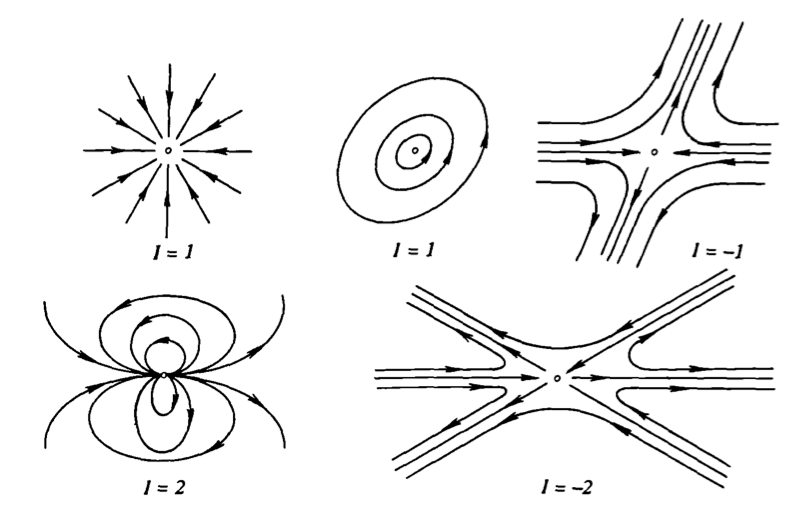
\includegraphics[width=0.8\textwidth]{img/IndiceCampos.png}
\caption{Índice de varios campos. Imagen de \cite[Fig. 6.1, p. 101]{doCarmo94}.}
\label{figIndiceCampos}
\end{figure}

El índice será 1, por ejemplo, si damos una vuelta alrededor del punto en el mismo sentido de la orientación. La imagen \ref{figIndiceCampos} muestra varios posibles campos con sus índices.

Hay que notar que durante la definición hemos hecho varias elecciones: de la curva, de la referencia y de la métrica. Antes de seguir, hemos de demostrar que el índice está efectivamente bien definido.

\begin{lemma} El índice no depende de la curva $C$ escogida siempre que sea topológicamente una circunferencia y contenga únicamente al punto singular $p$.
\end{lemma}

\begin{proof} Si cogemos $I_1, I_2$ los índices dados por dos curvas $C_1, C_2$, vemos que \[ I_1 - I_2 = \frac{1}{2π} \int_{C_1} τ - \frac{1}{2π} \int_{C_2} τ \eqexpl{Stokes} \frac{1}{2π} \int_Δ \dif τ = 0\] donde $Δ$ es la región encerrada entre $C_2$ y $C_1$, ya que $\dif τ = 0$.
\end{proof}

\begin{lemma} El índice no depende de la métrica Riemanniana escogida.
\end{lemma}

\begin{proof} Para esta demostración vamos a hacer un truco que es una demostración de la métrica. Definimos dos métricas $\pesc{·,·}_1$, $\pesc{·,·}_2$. Tomamos entonces el segmento que une ambas métricas, cosa que podemos hacer porque las métricas son un espacio vectorial de tensores. Definimos entonces  \[ \pesc{·,·}_t = t \pesc{·,·}_1 + (1-t)\pesc{·,·}_2 \] con $t∈[0,1]$

Es fácil ver que $\pesc{·,·}_t$ es Riemanniana si las dos de antes son Riemannianas. Definimos entonces índices $I_t, I_1, I_2$ con respecto a cada métrica respectivamente.

Por el lema anterior, es fácil ver que $I_t$ va a depender continuamente de $t$. Ahora la conclusión es inmediata: si $I_t$ es continua y valora en los enteros, sólo puede ser constante.
\end{proof}

\begin{lemma} El índice no depende de la referencia tomada $\set{e_1, e_2}$ que nos da las formas $ω_1, ω_2, ω_{12}$.
\end{lemma}

\begin{proof} Consideramos $p$ y una circunferencia estándar $S_r$ en la carta. Suponemos $p = (0,0)$ en la carta. La circunferencia encerrará una bola de radio $r$ $\bola_r$. Calculamos el límite siguiente \( \lim_{r\to 0} \frac{1}{2π} \int_{S_r} \gor{ω}_{12} ≝ \gor{I} \label{eqProofRef1} \)

Además, vamos a tratar de demostrar que $I = \gor{I}$, esto es, que el índice no depende de la referencia tomada $\set{e_1, e_2}$ sino más bien de la referencia $\set{\gor{e}_1, \gor{e}_2}$ que construimos a partir del vector.

Para demostrar que existe el límite, consideramos la sucesión de números reales $\int_{S_{r_i}} \gor{ω}_{12}$ y vemos que es de Cauchy. Evaluamos la diferencia \( \int_{S_{r_1}} \gor{ω}_{12} - \int_{S_{r_2}} \gor{ω}_{12} \eqexpl{Stokes} \int_Δ \dif \gor{ω}_{12} \label{eqProofRef2} \), donde de nuevo $Δ$ es la región encerrada por las dos curvas $S_{r_1}, S_{r_2}$. Cuando hacemos tender $r_1, r_2 \to 0$, es claro que esa integral se va a cero. Luego la sucesión es de Cauchy y el límite existe.

Ahora hay que ver que el límite es igual al índice. Para eso fijamos un $r_1$ y hacemos tender $r_2$ a 0 en \eqref{eqProofRef2} y tenemos que \( \lim_{r_2 \to 0}  \int_{S_{r_1}} \gor{ω}_{12} - \int_{S_{r_2}} \gor{ω}_{12} = \int_{S_{r_1}} \gor{ω}_{12} - 2π\gor{I} \label{eqProofRef3} \) usando \eqref{eqProofRef1} para decir que $\lim_{r_2\to 0} \int_{S_{r_2}} \gor{ω}_{12} = 2π\gor{I}$.

Pero también podemos aplicar Stokes en \eqref{eqProofRef2} y nos queda que
\(
	\lim_{r_2 \to 0}  \int_{S_{r_1}} \gor{ω}_{12} - \int_{S_{r_2}} \gor{ω}_{12} \eqexpl{Stokes}
	\int_{\bola_{r_1}} \dif \gor{ω}_{12} - \lim_{r_2 \to 0} \underbracket{\int_{\bola_{r_2}}\dif \gor{ω}_{12}}_{\to 0} =
	\int_{\bola_{r_1}} \dif \gor{ω}_{12}
	\label{eqProofRef4}
\)

Juntando \eqref{eqProofRef3} y \eqref{eqProofRef4}, nos queda \( \int_{S_{r_1}} \gor{ω}_{12} = \int_{\bola_{r_1}} \dif \gor{ω}_{12} + 2π\gor{I} \label{eqProofRef5} \)

Por otra parte, usando ahora la fórmula del lema \ref{thmOmegaTau} que nos decía que $\gor{ω}_{12} = ω_{12} + τ$, tenemos que \( \int_{S_{r_1}} \gor{ω}_{12} = \int_{S_{r_1}} ω_{12} + \int_{S_{r_1}} τ \eqexpl{Stokes} \int_{\bola_{r_1}} \dif ω_{12} + \int_{S_{r_1}} τ = \int_{\bola_{r_1}} \dif ω_{12}  + 2πI \label{eqProofRef6}\)

Hemos encontrado dos expresiones diferentes para $\int_{S_{r_1}} \gor{ω}_{12}$ en \eqref{eqProofRef5} y \eqref{eqProofRef6}. Si tenemos en cuenta que $\dif τ = 0$, entonces $\dif ω_{12} = \dif \gor{ω}_{12}$. Sólo nos queda rematar: \begin{align*}
\int_{S_{r_1}} \gor{ω}_{12} &= \int_{S_{r_1}} \gor{ω}_{12} \\
\int_{\bola_{r_1}} \dif \gor{ω}_{12} + 2π\gor{I} &= \int_{\bola_{r_1}} \dif ω_{12}  + 2πI \\
2π\gor{I} &= 2πI \\
\gor{I} &= I
\end{align*} y ya tenemos demostrado lo que queríamos\footnote{En \cite[p.101]{doCarmo94} comenta que $\gor{ω}_{12}$ no está definido en todo $\bola_{r_2}$ pero sí que lo está $K \gor{ω}_1 ∧ \gor{ω}_2$, pero no acabo de ver por qué sí puede usar tranquilamente $\gor{ω}_1$. Así que, por no complicarme la vida he dejado ahí $\dif ω_{12}$ sin preocuparme demasiado, supongo que usando cosas parecidas a las de la sección \ref{secIndependenciaEcsEstructura} se podrá llegar a algo que esté bien definido.}.
\end{proof}

Una parte que hemos probado en esta demostración nos vendrá muy bien para luego, así que nos la dejamos como corolario.

\begin{corol} Dado un campo $X$ con punto singular $p$ en una superficie $M$, consideramos en $U\setminus\set{p} ⊂ M$ una referencia dada por $\gor{e}_1 ≝ \frac{X}{\md{X}}$ y el vector $\gor{e}_2$ que completa la referencia ortonormal y mantiene la orientación. Calculamos también la correspondiente forma de la ecuación de estructura $\gor{ω}_{12}$.

Entonces, se tiene que el índice de $X$ en $p$ es \[ I_p(X) = \lim_{r \to 0} \frac{1}{2π} \int_{S_r} \gor{ω}_{12} \] donde $S_r$ es la circunferencia de radio $r$ centrada en $p$.
\end{corol}

¿Qué significado tiene este corolario? En el fondo no es más que seguir con la definición de índice que dábamos antes: $\gor{ω}_{12}$ nos dice para dónde cambia el vector $\gor{e}_1$ de la base. Si la referencia da ``dos vueltas'', entonces $\gor{ω}_{12}$ también dará ``dos vueltas''. La ventaja es que esta vez lo hemos hecho de tal forma que hemos llegado a algo que puede ser muy interesante, porque nos hemos ido al mundo de las ecuaciones de estructura, que ya vimos en \ref{secIndependenciaEcsEstructura} que son independientes de la referencia tomada. Es tan interesante que de hecho tenemos un teorema muy importante:

\begin{theorem}[Teorema\IS de Gauss-Bonnet] Sea $M$ una variedad diferenciable de dimensión dos, compacta y orientable. Sea $X$ un campo vectorial diferenciable con singularidades aisladas $p_1, \dotsc, p_k$. Entonces, para cualquier métrica Riemanniana en $M$, se tiene que
\[\frac{1}{2π} \int_M K ω_1 ∧ ω_2 = \sum_{p_i} I_{p_i}(X)\]
con $K$ la curvatura gaussiana.
\end{theorem}

\begin{proof}

Consideremos en $M^2 \setminus \bigcup \set{p_i}$ la referencia $\set{e_1 = \frac{X}{\md{X}}, e_2}$, donde $e_2$ es un campo de vectores unitario ortogonal a $e_1$ en la orientación de $M$.

Denotemos por $\bola_i$ una bola centrada en $p_i$ que no contiene ningún punto singular más que $p_i$. Por el teorema de Stokes tenemos que:

\[\int_{M-\bigcup \bola_i} K\bar{ω_1} ∧ \bar{ω_2} \eqexpl{\ref{eqCurvaturaGauss}} -\int_{M-\bigcup \bola_i} d\bar{ω}_{12} \overset{St} = \int_{∪d\bola_i}\bar{ω}_{12} = \sum \int_{∂\bola_i} \bar{ω}_{12} \]

donde $\partial \bola_i$ tiene la orientación inducida por $\bola_i$ (el contrario de la orientación de $M\setminus \bola_i$, de ahí el cambio de signo en la primera igualdad).

Ahora tomamos el límite de la igualdad superior cuando el radio de $\bola_i$ tiende a 0 obteniendo:
\[\int_M K ω_1 \y ω_2 = 2π \sum_i I_i\]

\end{proof}

La parte de la izquierda de la igualdad no depende del campo de vectores $X$ y la parte derecha no depende de la métrica. Por tanto podemos concluir que $\sum_i I_i$ es la misma para todos los campos de vectores con singularidades aisladas y que $\int_M Kσ$ es la misma para cualquier métrica Riemanniana en $M$. Es decir, que esto que hemos sacado es algún tipo de invariante de nuestra variedad $M$. Para ver qué es exactamente vamos a tener que profundizar un poco en topología.

\subsection{Cálculo del índice de un campo}

Antes de seguir, vamos a ver cómo calcular el índice de un campo. Hay algunas proposiciones que nos pueden ayudar, que saco de \cite[Sección 7.3]{barden03}.

\begin{prop} Sean $\appl{X}{U}{ℝ^m}$ y $\appl{Y}{V}{ℝ^m}$ dos campos de vectores cuyo único punto singular sea $p$ y tales que, para un cierto $δ > 0$, se tenga que $\restr{X}{\bola_δ(p)} = \restr{Y}{\bola_δ(p)}$. Entonces, $I(X, p) = I(Y, p)$.
\end{prop}

\begin{prop} Sean $\appl{X}{ℝ^m}{ℝ^m}$ y $\appl{Y}{ℝ^m}{ℝ^m}$ dos campos de vectores cuyo único punto singular sea $p$. Entonces, $X○Y$ es un campo vectorial y además $I(X○Y,p) = I(X,p) · I(Y,p)$.
\end{prop}

\begin{prop}  Sean $\appl{X}{ℝ^m}{ℝ^m}$ y $\appl{Y}{ℝ^m}{ℝ^m}$ dos campos de vectores cuyo único punto singular sea $p$. Si existe una homotopía de $X$ a $Y$ que fija el origen, entonces $I(X,p) = I(Y,p)$.
\end{prop}

\begin{prop} Sea $\appl{X}{ℝ^m}{ℝ^m}$ un isomorfismo lineal. Entonces, tratado como un campo vectorial, se tiene que $I(X, 0) = \sign(\det(X))$.
\end{prop}

\begin{prop} Sea $\appl{X}{ℝ^m}{ℝ^m}$ un campo vectorial con singularidad en el origen y para el cual $\Dif X(0)$ es no singular. Entonces $I(X,0) = \sign(\det(\Dif_0 X))$.
\end{prop}

\section{Triangulaciones y característica de Euler-Poincaré}

Vayámonos un poco a la topología. Si recordamos la geometría de poliedros, había una fórmula, llamada la fórmula de Euler, que nos decía que el número de vértices menos el de lados más el número de caras era siempre $2$. ¿Podemos extender eso a variedades diferenciables? La respuesta es que sí, y de hecho es un teorema bastante importante. Pero primero, tenemos que ver cómo podemos hablar de vértices y lados en algo que es suave y no es un poliedro.

\begin{defn}[Triangulación] Dada una variedad compacta $M$, se dice que una triangulación es una partición $\mathcal{T} = \set{T_i}$ de $M$ tal que $\bigcup T_i = M$, donde cada $T_i$ es difeomorfo a un triángulo (tres lados y tres vértices) y para la que se cumple que, dados $T_i ≠ T_j$, su intersección debe ser o bien vacía, o un vértice o un lado.
\end{defn}

\begin{defn}[Característica\IS de Euler-Poincaré]
Sea $M$ una variedad diferenciable y $\mathcal{T}$ una triangulación de $M$. Entonces, se tiene que \[ \chi(M) ≝ \#V - \#L + \#C ∈ℤ \] donde $V$ el número de vértices de la triangulación, $L$ el número de lados y $C$ el número de caras.
\end{defn}

Lo interesante de esta fórmula es que no depende de la triangulación elegida, sino de la topología.

Vamos a ver un par de ejemplos:

\begin{example}
Sea $M$ un tetraedro. Tenemos entonces $V=6,A=12,C=8$, con lo que la característica es $2$. Con esto, tenemos (si de verdad fuera topológico, que no lo hemos demostrado todavía) tendríamos que la característica de EP de la esfera es 2 (porque el tetraedro y la esfera son homeomorfos\footnote{Rafa dice que si ``hinchásemos'' el tetraedro como si de un globo se tratase, obtendríamos una esfera.})
\end{example}

\begin{example}

Vamos a ver la triangulación de un toro. Para ello, es pensamos en el toro como un cuadrado con los lados identificados. Construimos en ese cuadrado un triángulo rectángulo en una esquina y tiramos 4 paralelas a esa, de tal forma que la tercera sea la diagonal.

Así, tenemos $V=9$, $L=27$ y $C=18$. Para calcularlo tenemos que tener cuidado con las identificaciones (cada lado del cuadrado se identifica con el paralelo).
\end{example}


\begin{theorem}[Teorema\IS de Poincaré-Hopf]
Sea $D$ un campo en una variedad $M$. Entonces, se tiene que \[ \sum I_i(D) = χ(M) \]
\end{theorem}

Por el teorema de Gauss-Bonnet sabemos que la suma de los índices no depende del campo elegido. Eso es lo que nos va a dar la clave para que no dependa de la triangulación.

\begin{proof}
Esta demostración merece la pena mirarla en el doCarmo (Página 101) que hay unos dibujos de campos que se utilizan en la demostración de verdad al final de la página 103.

El esquema es probar que para toda triangulación se puede conseguir un campo que cumpla la fórmula.

Una vez tenemos ese campo construido (Fig 6.2 del doCarmo - página 104), por el teorema de Gauss-Bonnet, sabemos que la suma de los índices no depende del campo elegido.
\end{proof}

\section{Teorema de Gauss-Bonnet-Poincaré}

\begin{theorem}[Teorema\IS de Gauss-Bonnet-Poincaré]
Sea $M$ una variedad diferencial de dimensión dos, orientable y compacta, con frontera $\partial M$ y sea $X$ un campo de vectores en $M$ diferenciable y transversal a $\partial M$ (esto es, $X$ no es tangente en ningún punto a $\partial M$).

Supongamos que $p_1,...p_k$, singularidades de $X$, son aisladas y no se encuentran en $\partial M$ y sean $I_1,...,I_k$ sus índices respectivos.

Entonces, para cualquier métrica Riemanniana en $M$
\[\int_M Kσ + \int_{\partial M} k_g \dif s= 2π\sum I_{i}\]
donde $k_g$ es la curvatura geodésica de $\partial M$ y  $\dif s$ es el elemento de arco de $\partial M$
\end{theorem}

\begin{proof}
Tomemos una métrica Riemanniana en $M$ y consideremos en ella la referencia ortonormal orientada: $\bar{e}_1=X/|X|,\bar{e}_2$. Tomemos, en un entorno $V \subset M$ de $\partial M$ otra referencia orientada $\{e_1,e_2\}$ tal que, restringida a $\partial M$, $e_1$ es tangente a $\partial M$. Entonces
\[i^* \bar{ω}_{12}=i^*ω_{12}+\dif \psi\]
donde $\appl{i}{\partial M}{M}$ es la inclusión y $\psi$ es el ángulo entre $\bar{e}_1$ y $e_1$ en $\partial M$.

Sea $B_i$ una bola de centro $p_i$ para $i=1,...,k$ tal que no contiene ningún punto singular aparte de $p_i$. Entonces:
\[\int_{M - \cup B_i} K \bar{ω}_{1}\y \bar{ω}_2 = - \int_{M - \cup B_i} \dif \bar{ω}_{12} = \int_{\cup \partial B_i} \bar{ω}_{12}-\int_{\partial M}i^* \bar{ω}_{12}\]

por tanto
\[\int_{M - \cup B_i} K \bar{ω}_{1}\y \bar{ω}_2 + \int_{\partial M}i^* \bar{ω}_{12} = \sum_{i=1}^k \int_{\partial B_i} \bar{ω}_{12}\]

Por otro lado, por la definición de curvatura geodésica, tenemos
\[\int_{\partial M} i^*\bar{ω}_{12} = \int_{\partial M} i^*ω_{12}+\int_{\partial M} \dif \psi = \int_{\partial M}k_g \dif s + \int_{\partial M} \dif \psi\]

Como $\bar{e}_1=X/|X|$ no es tangente en ningún punto a $\partial M$, $\int_{\partial M}k_g \dif s=0$. Así, tomando el límite cuando el radio de $B_i$ tiende a 0 obtenemos:
\[\int_M K σ + \int_{\partial M} k_g \dif s = 2π \sum I_i\]
\end{proof}

\section{Conclusiones. Diatriba final.}
Aquí finaliza el curso. Nos hemos dejado el último punto del teorema que es la extensión a dimensiones infinitas de la referencia móvil, que es para lo que servía el álgebra multilineal.

Rafa se comenta que ahora siendo los cursos de 3 horas, hay asignaturas  que se quedan cojas. Nos pone el ejemplo de la teoría de Galois, que siendo sólo de 3 horas se queda corta y coja porque no se ven los teoremas realmente interesantes.

